\documentclass{article}\usepackage[]{graphicx}\usepackage[]{color}
%% maxwidth is the original width if it is less than linewidth
%% otherwise use linewidth (to make sure the graphics do not exceed the margin)
\makeatletter
\def\maxwidth{ %
  \ifdim\Gin@nat@width>\linewidth
    \linewidth
  \else
    \Gin@nat@width
  \fi
}
\makeatother

\definecolor{fgcolor}{rgb}{0.514, 0.58, 0.588}
\newcommand{\hlnum}[1]{\textcolor[rgb]{0.863,0.196,0.184}{#1}}%
\newcommand{\hlstr}[1]{\textcolor[rgb]{0.863,0.196,0.184}{#1}}%
\newcommand{\hlcom}[1]{\textcolor[rgb]{0.345,0.431,0.459}{#1}}%
\newcommand{\hlopt}[1]{\textcolor[rgb]{0.576,0.631,0.631}{#1}}%
\newcommand{\hlstd}[1]{\textcolor[rgb]{0.514,0.58,0.588}{#1}}%
\newcommand{\hlkwa}[1]{\textcolor[rgb]{0.796,0.294,0.086}{#1}}%
\newcommand{\hlkwb}[1]{\textcolor[rgb]{0.522,0.6,0}{#1}}%
\newcommand{\hlkwc}[1]{\textcolor[rgb]{0.796,0.294,0.086}{#1}}%
\newcommand{\hlkwd}[1]{\textcolor[rgb]{0.576,0.631,0.631}{#1}}%

\usepackage{framed}
\makeatletter
\newenvironment{kframe}{%
 \def\at@end@of@kframe{}%
 \ifinner\ifhmode%
  \def\at@end@of@kframe{\end{minipage}}%
  \begin{minipage}{\columnwidth}%
 \fi\fi%
 \def\FrameCommand##1{\hskip\@totalleftmargin \hskip-\fboxsep
 \colorbox{shadecolor}{##1}\hskip-\fboxsep
     % There is no \\@totalrightmargin, so:
     \hskip-\linewidth \hskip-\@totalleftmargin \hskip\columnwidth}%
 \MakeFramed {\advance\hsize-\width
   \@totalleftmargin\z@ \linewidth\hsize
   \@setminipage}}%
 {\par\unskip\endMakeFramed%
 \at@end@of@kframe}
\makeatother

\definecolor{shadecolor}{rgb}{.97, .97, .97}
\definecolor{messagecolor}{rgb}{0, 0, 0}
\definecolor{warningcolor}{rgb}{1, 0, 1}
\definecolor{errorcolor}{rgb}{1, 0, 0}
\newenvironment{knitrout}{}{} % an empty environment to be redefined in TeX

\usepackage{alltt}
\usepackage{geometry}
\geometry{verbose, tmargin=2.5cm, bmargin=2.5cm, lmargin=2.5cm, rmargin=2.5cm}
\IfFileExists{upquote.sty}{\usepackage{upquote}}{}
\begin{document}

\title{Data Extraction Evaluation}
\author{Matthew Leonawicz}
\maketitle





\section{Statistical sampling for spatial data extraction}

\subsection{Motivation: Data processing efficiency}

We've gotten faster at SNAP, but so has our need for speed. What was once never bothered with (outside some of my own work),
using statistical sampling to obtain results at no cost to validity, accuracy or precision compared to a census of our data,
is now more relevant than ever.
Before, we were content to let a process run in the background for hours and look at the results when done.
There was little incentive to incorporate techniques like those laid out here.
Now we have more types of data delivery and presentation, e.g., web applications, where it is intended for there to be a human watching and waiting for data processing to occur.

\subsubsection{Assumptions, bad ones}
An assumption I often encounter from those outside statistics, but involved in "big data" is that with today's processing power there is no reason not to use all the data.
A corollary of this is that many statistical methods can be dispensed with,
which is based on another assumption that this is what statistics basically exists for;
to help us hobble along when we were in the stone age.
However, both of these views are flawed.
The latter suggests little knowledge of the broad uses of statistics.
The former suggests little knowledge of statistics period, or the myriad ways data can be improperly analyzed and results interpreted.

\subsubsection{Speed not for speed's sake}
Making things go faster is perhaps the last area of application I would ever find for statistical methods,
and since not a lot of traditional statistical analysis occurs at SNAP I do not want those untrained in statistics to get the wrong impression that speed improvements are all statistics is really good for.
But it is relevant and beneficial in the context of some of our workflows, particularly my own.
But I am also not the only one extracting and processing large amounts of data at SNAP.
One use of statistics is data reduction.
This is what I aim for when needing to "get things done faster," not really the speed itself.
I'd rather see a decrease in computational time required for large data processing occur as a latent consequence of smart application of statistical methods than as something forced for its own sake.
I will outline a simple and extremely common case.

\subsection{Case study: sample mean}

Example of population mean vs. sample mean for a typical map of SNAP's Alaska-Canada 2-km downscaled data.
The sample mean converges in distribution to the population mean quite quickly.

\begin{knitrout}
\definecolor{shadecolor}{rgb}{0, 0.169, 0.212}\color{fgcolor}\begin{kframe}
\begin{alltt}
\hlstd{no.knit} \hlkwb{<-} \hlkwa{if} \hlstd{(}\hlstr{"knitr"} \hlopt \hlkwd{names}\hlstd{(}\hlkwd{sessionInfo}\hlstd{()}\hlopt{$}\hlstd{otherPkgs))} \hlnum{FALSE} \hlkwa{else} \hlnum{TRUE}
\hlkwd{library}\hlstd{(raster)}
\hlkwd{library}\hlstd{(microbenchmark)}
\hlkwd{library}\hlstd{(ggplot2)}
\hlkwd{library}\hlstd{(reshape2)}
\end{alltt}
\end{kframe}
\end{knitrout}

\begin{knitrout}
\definecolor{shadecolor}{rgb}{0, 0.169, 0.212}\color{fgcolor}\begin{kframe}
\begin{alltt}
\hlkwd{setwd}\hlstd{(}\hlstr{"C:/github/DataExtraction/data"}\hlstd{)}
\hlcom{# testfile <-}
\hlcom{# 'Z:/Base_Data/ALFRESCO_formatted/ALFRESCO_Master_Dataset/ALFRESCO_Model_Input_Datasets/AK_CAN_Inputs/Climate/gfdl_cm2_1/sresa2/tas/tas_mean_C_alf_ar4_gfdl_cm2_1_sresa2_01_2045.tif'}
\hlstd{testfile} \hlkwb{<-} \hlstr{"tas_mean_C_AR5_GFDL-CM3_rcp60_01_2062.tif"}

\hlstd{r} \hlkwb{<-} \hlkwd{readAll}\hlstd{(}\hlkwd{raster}\hlstd{(testfile))}  \hlcom{# force into memory so I/O time does not confound extraction time}
\hlstd{v} \hlkwb{<-} \hlkwd{getValues}\hlstd{(r)}  \hlcom{# numeric vector}
\hlstd{dat.ind} \hlkwb{<-} \hlkwd{Which}\hlstd{(}\hlopt{!}\hlkwd{is.na}\hlstd{(r),} \hlkwc{cells} \hlstd{= T)}
\hlstd{d} \hlkwb{<-} \hlstd{v[dat.ind]}  \hlcom{# numeric vector of data values (drop NAs)}
\hlstd{nd} \hlkwb{<-} \hlkwd{length}\hlstd{(dat.ind)}
\end{alltt}
\end{kframe}
\end{knitrout}

\begin{knitrout}
\definecolor{shadecolor}{rgb}{0, 0.169, 0.212}\color{fgcolor}\begin{kframe}
\begin{alltt}
\hlcom{# continue indexing v since this is how it will tend to occur in practice}
\hlcom{# take mean of all cells}
\hlkwd{mean}\hlstd{(v,} \hlkwc{na.rm} \hlstd{= T)}
\end{alltt}
\begin{verbatim}
## [1] -12.7623
\end{verbatim}
\begin{alltt}
\hlcom{# take mean of only the data cells}
\hlkwd{mean}\hlstd{(v[dat.ind])}
\end{alltt}
\begin{verbatim}
## [1] -12.7623
\end{verbatim}
\begin{alltt}
\hlcom{# take mean of only the data cells using sum and known length}
\hlkwd{sum}\hlstd{(v[dat.ind])}\hlopt{/}\hlstd{nd}
\end{alltt}
\begin{verbatim}
## [1] -12.7623
\end{verbatim}
\begin{alltt}
\hlcom{# take mean of data cells with .Internal}
\hlkwd{.Internal}\hlstd{(}\hlkwd{mean}\hlstd{(v[dat.ind]))}
\end{alltt}
\begin{verbatim}
## [1] -12.7623
\end{verbatim}
\begin{alltt}
\hlcom{# take mean of data cells with .Internal sum, known length}
\hlkwd{.Primitive}\hlstd{(}\hlstr{"sum"}\hlstd{)(v[dat.ind])}\hlopt{/}\hlstd{nd}
\end{alltt}
\begin{verbatim}
## [1] -12.7623
\end{verbatim}
\end{kframe}
\end{knitrout}

\begin{knitrout}
\definecolor{shadecolor}{rgb}{0, 0.169, 0.212}\color{fgcolor}\begin{kframe}
\begin{alltt}
\hlstd{mean.pop} \hlkwb{<-} \hlkwd{sum}\hlstd{(d)}\hlopt{/}\hlstd{nd}
\hlstd{mean.pop.out} \hlkwb{<-} \hlkwd{round}\hlstd{(mean.pop,} \hlnum{1}\hlstd{)}  \hlcom{# round to one decimal place for temperature data}
\hlstd{discrete.out} \hlkwb{<-} \hlkwd{round}\hlstd{(}\hlkwd{seq}\hlstd{(mean.pop, mean.pop} \hlopt{+} \hlnum{0.4}\hlstd{,} \hlkwc{by} \hlstd{=} \hlnum{0.1}\hlstd{)} \hlopt{-} \hlnum{0.2}\hlstd{,} \hlnum{1}\hlstd{)}
\hlcom{# median.pop <- median(d) median.pop.out <- round(median.pop, 1) # round to}
\hlcom{# one decimal place for temperature data}
\hlstd{bounds.round} \hlkwb{<-} \hlstd{mean.pop.out} \hlopt{+} \hlkwd{c}\hlstd{(}\hlopt{-}\hlnum{0.05}\hlstd{,} \hlnum{0.05}\hlstd{)}  \hlcom{# within rounding distance of the rounded population mean}
\hlstd{bounds.signif} \hlkwb{<-} \hlstd{mean.pop} \hlopt{+} \hlkwd{c}\hlstd{(}\hlopt{-}\hlnum{0.1}\hlstd{,} \hlnum{0.1}\hlstd{)}  \hlcom{# bounds on the unrounded population mean at the significant digits distance}
\hlcom{# Use sample mean}
\hlstd{n} \hlkwb{<-} \hlnum{1e+05}
\hlstd{m} \hlkwb{<-} \hlnum{100}
\hlstd{keep} \hlkwb{<-} \hlkwd{seq}\hlstd{(}\hlnum{1000}\hlstd{, n,} \hlkwc{by} \hlstd{=} \hlnum{1000}\hlstd{)}  \hlcom{# burn in and thin to facilitate visualization}

\hlkwd{set.seed}\hlstd{(}\hlnum{47}\hlstd{)}
\hlstd{d.sub} \hlkwb{<-} \hlkwd{replicate}\hlstd{(m,} \hlkwd{sample}\hlstd{(d, n,} \hlkwc{replace} \hlstd{= F))}
\hlstd{means} \hlkwb{<-} \hlkwd{data.frame}\hlstd{(}\hlnum{1}\hlopt{:}\hlstd{n, (}\hlnum{1}\hlopt{:}\hlstd{n)}\hlopt{/}\hlstd{nd,} \hlkwd{apply}\hlstd{(d.sub,} \hlnum{2}\hlstd{,} \hlkwa{function}\hlstd{(}\hlkwc{x}\hlstd{,} \hlkwc{n}\hlstd{)} \hlkwd{cumsum}\hlstd{(x)}\hlopt{/}\hlstd{(}\hlnum{1}\hlopt{:}\hlstd{n),}
    \hlkwc{n} \hlstd{= n))}
\hlkwd{names}\hlstd{(means)} \hlkwb{<-} \hlkwd{c}\hlstd{(}\hlstr{"Size"}\hlstd{,} \hlstr{"Percent_Sample"}\hlstd{,} \hlkwd{paste0}\hlstd{(}\hlstr{"Sample_"}\hlstd{,} \hlkwd{c}\hlstd{(}\hlkwd{paste0}\hlstd{(}\hlnum{0}\hlstd{,} \hlnum{0}\hlopt{:}\hlnum{9}\hlstd{),}
    \hlnum{10}\hlopt{:}\hlstd{m)[}\hlnum{1}\hlopt{:}\hlstd{m]))}
\hlstd{means} \hlkwb{<-} \hlstd{means[keep, ]}
\hlstd{p} \hlkwb{<-} \hlkwd{data.frame}\hlstd{(}\hlkwc{Size} \hlstd{= keep,} \hlkwc{Percent_Sample} \hlstd{= keep}\hlopt{/}\hlstd{nd,} \hlkwc{P_value} \hlstd{=} \hlnum{1} \hlopt{-} \hlkwd{apply}\hlstd{(means,}
    \hlnum{1}\hlstd{,} \hlkwa{function}\hlstd{(}\hlkwc{x}\hlstd{)} \hlkwd{length}\hlstd{(}\hlkwd{which}\hlstd{(x} \hlopt{>=} \hlstd{bounds.signif[}\hlnum{1}\hlstd{]} \hlopt{&} \hlstd{x} \hlopt{<} \hlstd{bounds.signif[}\hlnum{2}\hlstd{]))}\hlopt{/}\hlkwd{length}\hlstd{(x)))}
\hlstd{means} \hlkwb{<-} \hlkwd{melt}\hlstd{(means,} \hlkwc{id.vars} \hlstd{=} \hlkwd{c}\hlstd{(}\hlstr{"Size"}\hlstd{,} \hlstr{"Percent_Sample"}\hlstd{),} \hlkwc{variable.name} \hlstd{=} \hlkwd{c}\hlstd{(}\hlstr{"Sample"}\hlstd{),}
    \hlkwc{value.name} \hlstd{=} \hlstr{"Mean"}\hlstd{)}
\hlstd{p} \hlkwb{<-} \hlkwd{melt}\hlstd{(p,} \hlkwc{id.vars} \hlstd{=} \hlkwd{c}\hlstd{(}\hlstr{"Size"}\hlstd{,} \hlstr{"Percent_Sample"}\hlstd{),} \hlkwc{variable.name} \hlstd{=} \hlkwd{c}\hlstd{(}\hlstr{"Type"}\hlstd{),}
    \hlkwc{value.name} \hlstd{=} \hlstr{"Pval"}\hlstd{)}

\hlstd{clr} \hlkwb{<-} \hlkwd{c}\hlstd{(}\hlkwc{Samples} \hlstd{=} \hlstr{"gray"}\hlstd{,} \hlkwc{`Pop. mean +/- 1 sig. fig.`} \hlstd{=} \hlstr{"blue"}\hlstd{,} \hlkwc{`Rounded pop. mean`} \hlstd{=} \hlstr{"red"}\hlstd{,}
    \hlkwc{`Possible rounded values`} \hlstd{=} \hlstr{"black"}\hlstd{)}
\end{alltt}
\end{kframe}
\end{knitrout}

\begin{knitrout}
\definecolor{shadecolor}{rgb}{0, 0.169, 0.212}\color{fgcolor}\begin{kframe}
\begin{alltt}
\hlkwa{if} \hlstd{(no.knit)} \hlkwd{png}\hlstd{(}\hlstr{"../plots/mean_by_size.png"}\hlstd{,} \hlkwc{width} \hlstd{=} \hlnum{2000}\hlstd{,} \hlkwc{height} \hlstd{=} \hlnum{1600}\hlstd{,} \hlkwc{res} \hlstd{=} \hlnum{200}\hlstd{)}
\hlstd{g} \hlkwb{<-} \hlkwd{ggplot}\hlstd{(means,} \hlkwd{aes}\hlstd{(}\hlkwc{x} \hlstd{= Percent_Sample,} \hlkwc{y} \hlstd{= Mean,} \hlkwc{group} \hlstd{= Sample))} \hlopt{+} \hlkwd{theme_bw}\hlstd{()} \hlopt{+}
    \hlkwd{geom_line}\hlstd{(}\hlkwd{aes}\hlstd{(}\hlkwc{colour} \hlstd{=} \hlstr{"Samples"}\hlstd{))} \hlopt{+} \hlkwd{geom_hline}\hlstd{(}\hlkwd{aes}\hlstd{(}\hlkwc{yintercept} \hlstd{= d,} \hlkwc{colour} \hlstd{=} \hlstr{"Rounded pop. mean"}\hlstd{),}
    \hlkwc{data} \hlstd{=} \hlkwd{data.frame}\hlstd{(}\hlkwc{d} \hlstd{= mean.pop.out))} \hlopt{+} \hlkwd{geom_hline}\hlstd{(}\hlkwd{aes}\hlstd{(}\hlkwc{yintercept} \hlstd{= d,} \hlkwc{colour} \hlstd{=} \hlkwd{c}\hlstd{(}\hlstr{"Pop. mean +/- 1 sig. fig."}\hlstd{)),}
    \hlkwc{data} \hlstd{=} \hlkwd{data.frame}\hlstd{(}\hlkwc{d} \hlstd{= bounds.signif))} \hlopt{+} \hlkwd{geom_hline}\hlstd{(}\hlkwd{aes}\hlstd{(}\hlkwc{yintercept} \hlstd{= d,} \hlkwc{colour} \hlstd{=} \hlstr{"Possible rounded values"}\hlstd{),}
    \hlstd{,} \hlkwc{data} \hlstd{=} \hlkwd{data.frame}\hlstd{(}\hlkwc{d} \hlstd{= discrete.out[}\hlnum{2}\hlopt{:}\hlnum{5}\hlstd{]),} \hlkwc{linetype} \hlstd{=} \hlnum{2}\hlstd{)} \hlopt{+} \hlkwd{scale_colour_manual}\hlstd{(}\hlkwc{name} \hlstd{=} \hlstr{"hello"}\hlstd{,}
    \hlkwc{values} \hlstd{= clr)} \hlopt{+} \hlkwd{theme}\hlstd{(}\hlkwc{legend.position} \hlstd{=} \hlstr{"bottom"}\hlstd{)} \hlopt{+} \hlkwd{labs}\hlstd{(}\hlkwc{title} \hlstd{=} \hlstr{"Sample mean ~ sample size"}\hlstd{)}
\hlkwd{print}\hlstd{(g)}
\end{alltt}
\end{kframe}
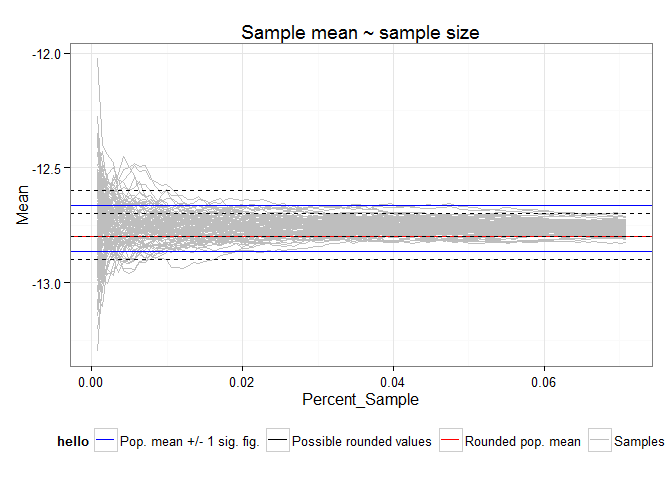
\includegraphics[width=\maxwidth]{figure/size-1} 
\begin{kframe}\begin{alltt}
\hlkwa{if} \hlstd{(no.knit)} \hlkwd{dev.off}\hlstd{()}
\end{alltt}
\end{kframe}
\end{knitrout}

\subsubsection{Justification}

The difference between sampling vs. using all data in a map layer is minimal.
It depends on various factors including but not limited to the statistic of interest, the spatial autocorrelation present in the map, and whether the entire map is of interest or just a particular region of a certain size.

In this example using the sample mean instead of the population mean, the difference is representative.
The difference is also not particularly meaningful.
It is also not final, as it tends to vanish anyway due to rounding to the nearest significant digits for the data after the statistic is computed.
The difference in means can also be bounded arbitrarily even without the rounding to significant digits performed at the end.

In the case of the mean we are helped out by the weak law of large numbers and the central limit theorem.
Consideration must also be given to the high level of spatial autocorrelation among pixels in the downscaled raster maps.
There is simply not as much data or information present as one might think and this drives the effective sample size.
 
\subsubsection{Results}

##### All points? No point.

Using the sample mean is helpful as a data reduction strategy while not being harmful in terms of representativeness.
The possible "tradeoff" itself appears to be largely a false dichotomy.
There is no benefit to computing the mean of all pixels in the example map layer.

##### How many samples do we really need?

\begin{knitrout}
\definecolor{shadecolor}{rgb}{0, 0.169, 0.212}\color{fgcolor}\begin{kframe}
\begin{alltt}
\hlkwa{if} \hlstd{(no.knit)} \hlkwd{png}\hlstd{(}\hlstr{"../plots/pvalue_sigdig.png"}\hlstd{,} \hlkwc{width} \hlstd{=} \hlnum{2000}\hlstd{,} \hlkwc{height} \hlstd{=} \hlnum{2000}\hlstd{,}
    \hlkwc{res} \hlstd{=} \hlnum{200}\hlstd{)}
\hlstd{g} \hlkwb{<-} \hlkwd{ggplot}\hlstd{(p,} \hlkwd{aes}\hlstd{(}\hlkwc{x} \hlstd{= Percent_Sample,} \hlkwc{y} \hlstd{= Pval,} \hlkwc{group} \hlstd{= Type,} \hlkwc{colour} \hlstd{= Type))} \hlopt{+}
    \hlkwd{theme_bw}\hlstd{()} \hlopt{+} \hlkwd{geom_line}\hlstd{(}\hlkwc{colour} \hlstd{=} \hlstr{"black"}\hlstd{)}
\hlstd{g} \hlkwb{<-} \hlstd{g} \hlopt{+} \hlkwd{geom_hline}\hlstd{(}\hlkwd{aes}\hlstd{(}\hlkwc{yintercept} \hlstd{=} \hlnum{0.05}\hlstd{,} \hlkwc{linetype} \hlstd{=} \hlstr{"P-value = 0.05"}\hlstd{),} \hlkwc{colour} \hlstd{=} \hlstr{"red"}\hlstd{,}
    \hlkwc{linetype} \hlstd{=} \hlnum{2}\hlstd{)} \hlopt{+} \hlkwd{annotate}\hlstd{(}\hlstr{"text"}\hlstd{,} \hlnum{0.005}\hlstd{,} \hlnum{0.05} \hlopt{*} \hlnum{1.2}\hlstd{,} \hlkwc{label} \hlstd{=} \hlstr{"P-value = 0.05"}\hlstd{,}
    \hlkwc{size} \hlstd{=} \hlnum{3}\hlstd{)}
\hlstd{g} \hlkwb{<-} \hlstd{g} \hlopt{+} \hlkwd{labs}\hlstd{(}\hlkwc{title} \hlstd{=} \hlstr{"P(abs(sample mean - pop. mean) > 1 sig. digit | sample size)"}\hlstd{)}
\hlkwd{print}\hlstd{(g)}
\end{alltt}
\end{kframe}
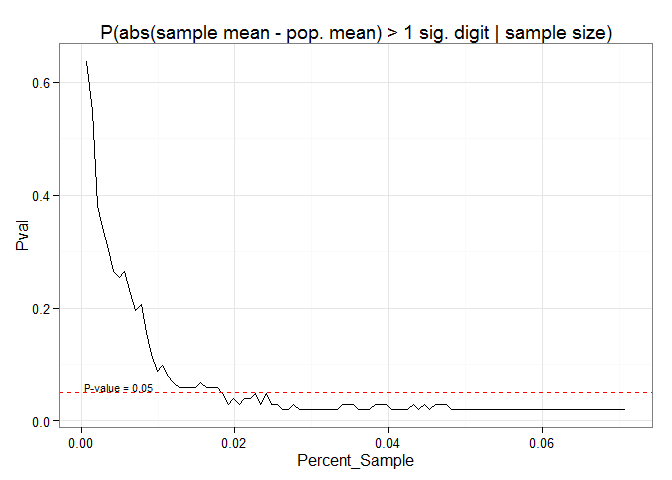
\includegraphics[width=\maxwidth]{figure/sigdig-1} 
\begin{kframe}\begin{alltt}
\hlkwa{if} \hlstd{(no.knit)} \hlkwd{dev.off}\hlstd{()}
\end{alltt}
\end{kframe}
\end{knitrout}

In this example even a two percent subsample of the original non-NA data cells is small enough to limit us to a five percent probability of obtaining a mean that differs from the mean computed on the full dataset
by an amount equal to or greater than the smallest discrete increment possible (0.1 degrees Celsius for SNAP temperature data) based simply on the number of significant figures present.
Furthermore, even for nominal sample sizes, the 0.05 probability is one almost strictly of minimal deviation (0.1 degrees).
The probability that a sample mean computed on a subsample of the map layer deviates enough from the population mean
to cause it to be rounded to two discrete incremental units from the population mean (0.2 degrees) is essentially zero (except if using crudely small sample sizes).

Although a two percent subsample appears sufficient for this criterion, let’s use a five percent subsample for illustration.
This is clearly overkill in this example since the p-value attenuates to the range of 0.019 to 0.029 by around 2.5 percent subsampling.

##### How much faster does this make things go?

Compute time for the mean is of course affected by the sample size.

\begin{knitrout}
\definecolor{shadecolor}{rgb}{0, 0.169, 0.212}\color{fgcolor}\begin{kframe}
\begin{alltt}
\hlcom{# compute time for means for different sample size}
\hlstd{s005pct} \hlkwb{<-} \hlstd{d.sub[}\hlnum{1}\hlopt{:}\hlkwd{round}\hlstd{((}\hlkwd{nrow}\hlstd{(d.sub)} \hlopt{*} \hlnum{0.05}\hlstd{)),} \hlnum{1}\hlstd{]}
\hlstd{s010pct} \hlkwb{<-} \hlstd{d.sub[}\hlnum{1}\hlopt{:}\hlkwd{round}\hlstd{((}\hlkwd{nrow}\hlstd{(d.sub)} \hlopt{*} \hlnum{0.1}\hlstd{)),} \hlnum{1}\hlstd{]}
\hlstd{s025pct} \hlkwb{<-} \hlstd{d.sub[}\hlnum{1}\hlopt{:}\hlkwd{round}\hlstd{((}\hlkwd{nrow}\hlstd{(d.sub)} \hlopt{*} \hlnum{0.25}\hlstd{)),} \hlnum{1}\hlstd{]}
\hlstd{s100pct} \hlkwb{<-} \hlstd{d.sub[,} \hlnum{1}\hlstd{]}
\end{alltt}
\end{kframe}
\end{knitrout}

\begin{knitrout}
\definecolor{shadecolor}{rgb}{0, 0.169, 0.212}\color{fgcolor}\begin{kframe}
\begin{alltt}
\hlstd{mb3} \hlkwb{<-} \hlkwd{microbenchmark}\hlstd{(}\hlkwd{sum}\hlstd{(s005pct)}\hlopt{/}\hlkwd{length}\hlstd{(s005pct),} \hlkwd{sum}\hlstd{(s010pct)}\hlopt{/}\hlkwd{length}\hlstd{(s010pct),}
    \hlkwd{sum}\hlstd{(s025pct)}\hlopt{/}\hlkwd{length}\hlstd{(s025pct),} \hlkwd{sum}\hlstd{(s100pct)}\hlopt{/}\hlkwd{length}\hlstd{(s100pct),} \hlkwc{times} \hlstd{=} \hlnum{10000}\hlstd{)}
\hlstd{mb3}
\end{alltt}
\begin{verbatim}
## Unit: microseconds
##                          expr    min     lq      mean median     uq
##  sum(s005pct)/length(s005pct)  4.976  5.288  5.329049  5.288  5.288
##  sum(s010pct)/length(s010pct)  9.642  9.642  9.919523  9.953  9.953
##  sum(s025pct)/length(s025pct) 23.326 23.326 23.703385 23.637 23.637
##  sum(s100pct)/length(s100pct) 91.746 92.057 92.653782 92.057 92.058
##      max neval
##   48.828 10000
##   77.440 10000
##  163.899 10000
##  807.050 10000
\end{verbatim}
\begin{alltt}
\hlkwa{if} \hlstd{(no.knit)} \hlkwd{png}\hlstd{(}\hlstr{"../plots/benchmark3.png"}\hlstd{,} \hlkwc{width} \hlstd{=} \hlnum{2000}\hlstd{,} \hlkwc{height} \hlstd{=} \hlnum{1600}\hlstd{,} \hlkwc{res} \hlstd{=} \hlnum{200}\hlstd{)}
\hlkwd{autoplot}\hlstd{(mb3)} \hlopt{+} \hlkwd{theme_bw}\hlstd{()} \hlopt{+} \hlkwd{labs}\hlstd{(}\hlkwc{title} \hlstd{=} \hlstr{"Compute time for mean by sample size"}\hlstd{,}
    \hlkwc{y} \hlstd{=} \hlstr{"Function"}\hlstd{)}
\end{alltt}
\end{kframe}
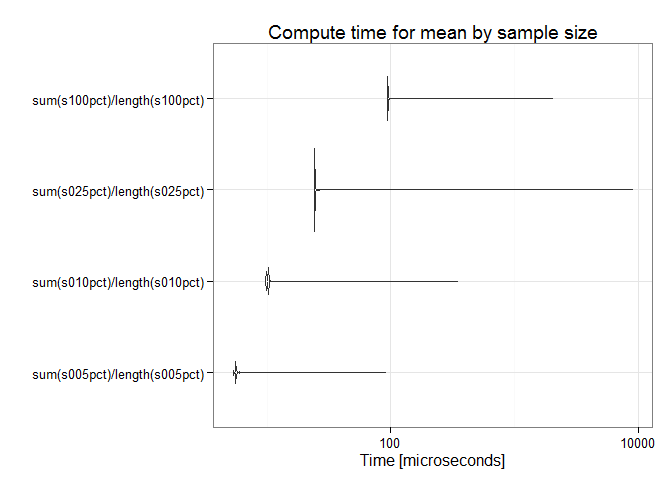
\includegraphics[width=\maxwidth]{figure/benchmarks3-1} 
\begin{kframe}\begin{alltt}
\hlkwa{if} \hlstd{(no.knit)} \hlkwd{dev.off}\hlstd{()}
\end{alltt}
\end{kframe}
\end{knitrout}

Using optimal subsampling to estimate the mean achieves speed improvements orders of magnitude greater than what can be achieved through strictly algorithmic changes to how the mean is computed on the full dataset,
though those help immensely as well, also by many orders of magnitude.
Sampling is vastly more effective, but both approaches can be combined for maximum benefit.

\begin{knitrout}
\definecolor{shadecolor}{rgb}{0, 0.169, 0.212}\color{fgcolor}\begin{kframe}
\begin{alltt}
\hlstd{mb4} \hlkwb{<-} \hlkwd{microbenchmark}\hlstd{(}\hlkwd{sum}\hlstd{(s005pct)}\hlopt{/}\hlkwd{length}\hlstd{(s005pct),} \hlkwd{mean}\hlstd{(v,} \hlkwc{na.rm} \hlstd{= T),} \hlkwd{sum}\hlstd{(d)}\hlopt{/}\hlkwd{length}\hlstd{(d),}
    \hlkwd{mean}\hlstd{(s005pct),} \hlkwc{times} \hlstd{=} \hlnum{100}\hlstd{)}
\hlstd{mb4}
\end{alltt}
\begin{verbatim}
## Unit: microseconds
##                          expr        min          lq         mean
##  sum(s005pct)/length(s005pct)      4.977      6.9985     10.33559
##            mean(v, na.rm = T) 391108.905 394197.6155 401290.90893
##              sum(d)/length(d)   1476.325   1482.7000   1497.67516
##                 mean(s005pct)     17.417     19.7500     45.08691
##      median         uq        max neval
##       9.331     10.575     19.283   100
##  395102.475 408130.325 504864.841   100
##    1488.765   1498.095   1663.236   100
##      54.271     62.512     68.421   100
\end{verbatim}
\begin{alltt}
\hlstd{med} \hlkwb{<-} \hlkwd{print}\hlstd{(mb4)}\hlopt{$}\hlstd{median}
\end{alltt}
\begin{verbatim}
## Unit: microseconds
##                          expr        min          lq         mean
##  sum(s005pct)/length(s005pct)      4.977      6.9985     10.33559
##            mean(v, na.rm = T) 391108.905 394197.6155 401290.90893
##              sum(d)/length(d)   1476.325   1482.7000   1497.67516
##                 mean(s005pct)     17.417     19.7500     45.08691
##      median         uq        max neval
##       9.331     10.575     19.283   100
##  395102.475 408130.325 504864.841   100
##    1488.765   1498.095   1663.236   100
##      54.271     62.512     68.421   100
\end{verbatim}
\begin{alltt}
\hlkwd{names}\hlstd{(med)} \hlkwb{<-} \hlkwd{print}\hlstd{(mb4)}\hlopt{$}\hlstd{expr}
\end{alltt}
\begin{verbatim}
## Unit: microseconds
##                          expr        min          lq         mean
##  sum(s005pct)/length(s005pct)      4.977      6.9985     10.33559
##            mean(v, na.rm = T) 391108.905 394197.6155 401290.90893
##              sum(d)/length(d)   1476.325   1482.7000   1497.67516
##                 mean(s005pct)     17.417     19.7500     45.08691
##      median         uq        max neval
##       9.331     10.575     19.283   100
##  395102.475 408130.325 504864.841   100
##    1488.765   1498.095   1663.236   100
##      54.271     62.512     68.421   100
\end{verbatim}
\begin{alltt}
\hlstd{med} \hlkwb{<-} \hlstd{med[}\hlkwd{c}\hlstd{(}\hlnum{1}\hlstd{,} \hlnum{4}\hlopt{:}\hlnum{2}\hlstd{)]}

\hlkwa{if} \hlstd{(no.knit)} \hlkwd{png}\hlstd{(}\hlstr{"../plots/benchmark4.png"}\hlstd{,} \hlkwc{width} \hlstd{=} \hlnum{2000}\hlstd{,} \hlkwc{height} \hlstd{=} \hlnum{1600}\hlstd{,} \hlkwc{res} \hlstd{=} \hlnum{200}\hlstd{)}
\hlkwd{autoplot}\hlstd{(mb4)} \hlopt{+} \hlkwd{theme_bw}\hlstd{()} \hlopt{+} \hlkwd{labs}\hlstd{(}\hlkwc{title} \hlstd{=} \hlstr{"Compute time for mean | sampling and/or function change"}\hlstd{,}
    \hlkwc{y} \hlstd{=} \hlstr{"Function"}\hlstd{)}
\end{alltt}
\end{kframe}
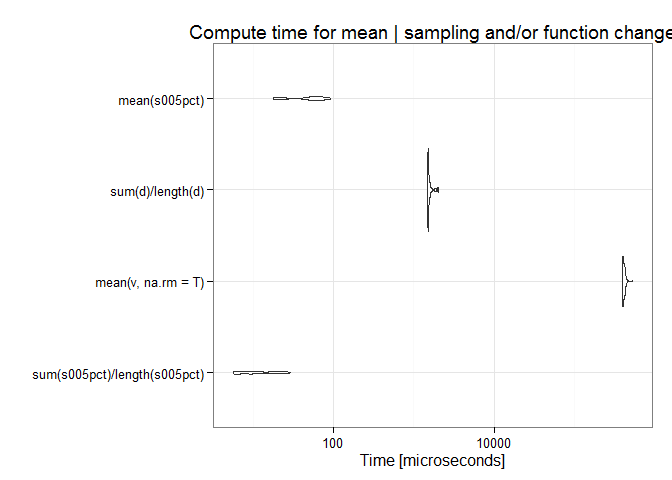
\includegraphics[width=\maxwidth]{figure/benchmarks4-1} 
\begin{kframe}\begin{alltt}
\hlkwa{if} \hlstd{(no.knit)} \hlkwd{dev.off}\hlstd{()}
\end{alltt}
\end{kframe}
\end{knitrout}

Similar to above, below are the median compute times for the mean using (1) the full data while removing NAs, (2) the sum divided by the length after NAs removed, (3) the mean of a subsample, and (4) a combination of (2) and (3).

\begin{knitrout}
\definecolor{shadecolor}{rgb}{0, 0.169, 0.212}\color{fgcolor}\begin{kframe}
\begin{alltt}
\hlkwa{if} \hlstd{(no.knit)} \hlkwd{png}\hlstd{(}\hlstr{"../plots/benchmark4medians.png"}\hlstd{,} \hlkwc{width} \hlstd{=} \hlnum{2000}\hlstd{,} \hlkwc{height} \hlstd{=} \hlnum{1000}\hlstd{,}
    \hlkwc{res} \hlstd{=} \hlnum{200}\hlstd{)}
\hlkwd{ggplot}\hlstd{(}\hlkwd{data.frame}\hlstd{(}\hlkwc{x} \hlstd{=} \hlkwd{names}\hlstd{(med),} \hlkwc{y} \hlstd{= med),} \hlkwd{aes}\hlstd{(}\hlkwc{x} \hlstd{=} \hlkwd{reorder}\hlstd{(x,} \hlnum{1}\hlopt{:}\hlkwd{length}\hlstd{(x),}
    \hlkwa{function}\hlstd{(}\hlkwc{z}\hlstd{) z),} \hlkwc{y} \hlstd{= y,} \hlkwc{colour} \hlstd{= x))} \hlopt{+} \hlkwd{geom_bar}\hlstd{(}\hlkwc{stat} \hlstd{=} \hlstr{"identity"}\hlstd{,} \hlkwc{size} \hlstd{=} \hlnum{0.5}\hlstd{,}
    \hlkwc{width} \hlstd{=} \hlnum{0.9}\hlstd{)} \hlopt{+} \hlkwd{theme_bw}\hlstd{()} \hlopt{+} \hlkwd{theme}\hlstd{(}\hlkwc{legend.position} \hlstd{=} \hlstr{"none"}\hlstd{,} \hlkwc{axis.ticks} \hlstd{=} \hlkwd{element_blank}\hlstd{(),}
    \hlkwc{axis.text.y} \hlstd{=} \hlkwd{element_blank}\hlstd{())} \hlopt{+} \hlkwd{scale_colour_manual}\hlstd{(}\hlkwc{values} \hlstd{=} \hlkwd{c}\hlstd{(}\hlstr{"gray"}\hlstd{,}
    \hlstr{"dodgerblue"}\hlstd{,} \hlstr{"orange"}\hlstd{,} \hlstr{"purple"}\hlstd{)[}\hlkwd{c}\hlstd{(}\hlnum{3}\hlstd{,} \hlnum{1}\hlstd{,} \hlnum{2}\hlstd{,} \hlnum{4}\hlstd{)])} \hlopt{+} \hlkwd{labs}\hlstd{(}\hlkwc{title} \hlstd{=} \hlstr{"Compute time for mean | sampling and/or function change"}\hlstd{,}
    \hlkwc{x} \hlstd{=} \hlstr{"Function +/- sampling"}\hlstd{,} \hlkwc{y} \hlstd{=} \hlstr{"Time [microseconds]"}\hlstd{)} \hlopt{+} \hlkwd{annotate}\hlstd{(}\hlstr{"text"}\hlstd{,}
    \hlkwc{x} \hlstd{= (}\hlnum{1}\hlopt{:}\hlnum{4}\hlstd{)} \hlopt{-} \hlnum{0.2}\hlstd{,} \hlkwc{y} \hlstd{=} \hlnum{20000}\hlstd{,} \hlkwc{label} \hlstd{=} \hlkwd{names}\hlstd{(med),} \hlkwc{size} \hlstd{=} \hlnum{4}\hlstd{,} \hlkwc{hjust} \hlstd{=} \hlnum{0}\hlstd{,} \hlkwc{colour} \hlstd{=} \hlkwd{c}\hlstd{(}\hlkwd{rep}\hlstd{(}\hlstr{"black"}\hlstd{,}
        \hlnum{3}\hlstd{),} \hlstr{"white"}\hlstd{))} \hlopt{+} \hlkwd{coord_flip}\hlstd{()}
\end{alltt}
\end{kframe}
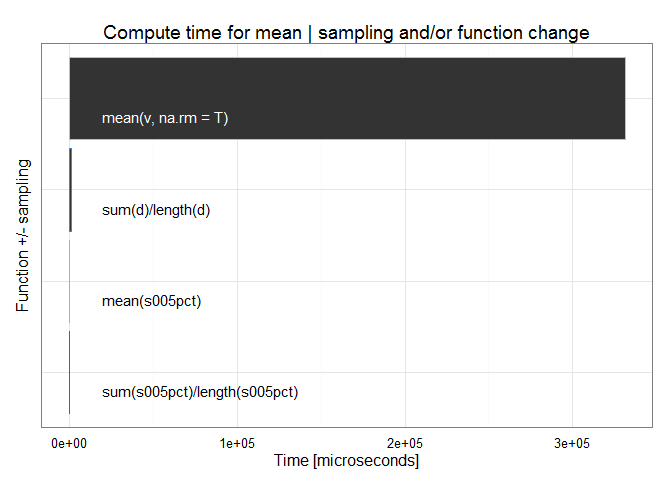
\includegraphics[width=\maxwidth]{figure/benchmarks4med1-1} 
\begin{kframe}\begin{alltt}
\hlkwa{if} \hlstd{(no.knit)} \hlkwd{dev.off}\hlstd{()}
\end{alltt}
\end{kframe}
\end{knitrout}

Here is the same plot after removing the first bar to better show the relative compute time for the other three methods.

\begin{knitrout}
\definecolor{shadecolor}{rgb}{0, 0.169, 0.212}\color{fgcolor}\begin{kframe}
\begin{alltt}
\hlkwa{if} \hlstd{(no.knit)} \hlkwd{png}\hlstd{(}\hlstr{"../plots/benchmark4medians2.png"}\hlstd{,} \hlkwc{width} \hlstd{=} \hlnum{2000}\hlstd{,} \hlkwc{height} \hlstd{=} \hlnum{1000}\hlstd{,}
    \hlkwc{res} \hlstd{=} \hlnum{200}\hlstd{)}
\hlkwd{ggplot}\hlstd{(}\hlkwd{data.frame}\hlstd{(}\hlkwc{x} \hlstd{=} \hlkwd{names}\hlstd{(med)[}\hlopt{-}\hlnum{4}\hlstd{],} \hlkwc{y} \hlstd{= med[}\hlopt{-}\hlnum{4}\hlstd{]),} \hlkwd{aes}\hlstd{(}\hlkwc{x} \hlstd{=} \hlkwd{reorder}\hlstd{(x,} \hlnum{1}\hlopt{:}\hlkwd{length}\hlstd{(x),}
    \hlkwa{function}\hlstd{(}\hlkwc{z}\hlstd{) z),} \hlkwc{y} \hlstd{= y,} \hlkwc{colour} \hlstd{= x))} \hlopt{+} \hlkwd{geom_bar}\hlstd{(}\hlkwc{stat} \hlstd{=} \hlstr{"identity"}\hlstd{,} \hlkwc{size} \hlstd{=} \hlnum{0.5}\hlstd{,}
    \hlkwc{width} \hlstd{=} \hlnum{0.9}\hlstd{)} \hlopt{+} \hlkwd{theme_bw}\hlstd{()} \hlopt{+} \hlkwd{theme}\hlstd{(}\hlkwc{legend.position} \hlstd{=} \hlstr{"none"}\hlstd{,} \hlkwc{axis.ticks} \hlstd{=} \hlkwd{element_blank}\hlstd{(),}
    \hlkwc{axis.text.y} \hlstd{=} \hlkwd{element_blank}\hlstd{())} \hlopt{+} \hlkwd{scale_colour_manual}\hlstd{(}\hlkwc{values} \hlstd{=} \hlkwd{c}\hlstd{(}\hlstr{"dodgerblue"}\hlstd{,}
    \hlstr{"orange"}\hlstd{,} \hlstr{"purple"}\hlstd{)[}\hlkwd{c}\hlstd{(}\hlnum{2}\hlstd{,} \hlnum{1}\hlstd{,} \hlnum{3}\hlstd{)])} \hlopt{+} \hlkwd{labs}\hlstd{(}\hlkwc{title} \hlstd{=} \hlstr{"Compute time for mean | sampling and/or function change"}\hlstd{,}
    \hlkwc{x} \hlstd{=} \hlstr{"Function +/- sampling"}\hlstd{,} \hlkwc{y} \hlstd{=} \hlstr{"Time [microseconds]"}\hlstd{)} \hlopt{+} \hlkwd{annotate}\hlstd{(}\hlstr{"text"}\hlstd{,}
    \hlkwc{x} \hlstd{= (}\hlnum{1}\hlopt{:}\hlstd{(}\hlnum{4} \hlopt{-} \hlnum{1}\hlstd{))} \hlopt{-} \hlnum{0.2}\hlstd{,} \hlkwc{y} \hlstd{=} \hlnum{125}\hlstd{,} \hlkwc{label} \hlstd{=} \hlkwd{names}\hlstd{(med)[}\hlopt{-}\hlnum{4}\hlstd{],} \hlkwc{size} \hlstd{=} \hlnum{4}\hlstd{,} \hlkwc{hjust} \hlstd{=} \hlnum{0}\hlstd{,}
    \hlkwc{colour} \hlstd{=} \hlkwd{c}\hlstd{(}\hlkwd{rep}\hlstd{(}\hlstr{"black"}\hlstd{,} \hlnum{3} \hlopt{-} \hlnum{1}\hlstd{),} \hlstr{"white"}\hlstd{))} \hlopt{+} \hlkwd{coord_flip}\hlstd{()}
\end{alltt}
\end{kframe}
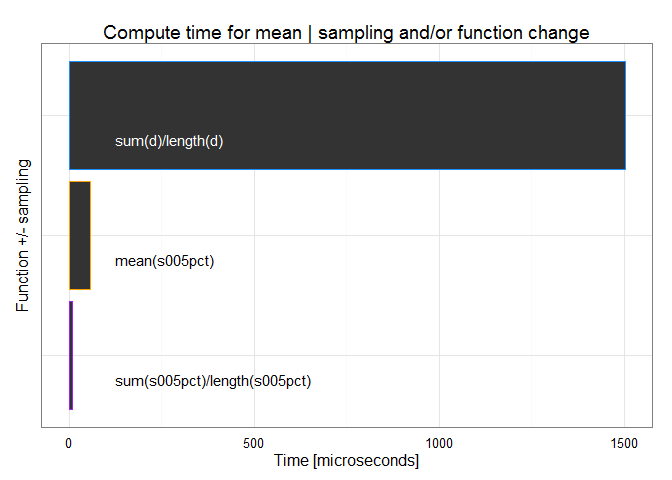
\includegraphics[width=\maxwidth]{figure/benchmarks4med2-1} 
\begin{kframe}\begin{alltt}
\hlkwa{if} \hlstd{(no.knit)} \hlkwd{dev.off}\hlstd{()}
\end{alltt}
\end{kframe}
\end{knitrout}

How does the benefit extend to extractions on maps at different extents, data heterogeneity, climate variables,
or for other common statistics such as the standard deviation?
These are open questions at the moment, but for one thing,
I expect more samples are needed for precipitation than temperature.
I also expect more samples needed to estimate parameters with higher moments.

\subsection{Next steps}

Combining sampling and data reduction methods while using the most efficient \textbf{R} functions can be particularly useful when processing large numbers of high-resolution geotiff raster layers.
One thing I already do when extracting from many files by shapefile is I avoid extracting by shape more than once.
I do it one time to obtain the corresponding raster layer cell indices.
Then on all subsequent maps I extract by cell indices which is notably faster.
Ultimately, there is much more room for speed improvements in terms of efficient use of statistics than in strictly programmatic corner-cutting.

The plots below benchmark different sample mean computations.
Comparisons involve the sample mean of the entire data set and do not involve the main approach outlined above which focuses on efficiency gains by taking the mean of a smaller, representative sample.
This provides some insight into how it is beneficial nonetheless to considering the right programmatic approach in conjunction with statistical efficiencies.

\begin{knitrout}
\definecolor{shadecolor}{rgb}{0, 0.169, 0.212}\color{fgcolor}\begin{kframe}
\begin{alltt}
\hlstd{mb} \hlkwb{<-} \hlkwd{microbenchmark}\hlstd{(}\hlkwd{mean}\hlstd{(v,} \hlkwc{na.rm} \hlstd{= T),} \hlkwd{mean}\hlstd{(v[dat.ind]),} \hlkwd{sum}\hlstd{(v[dat.ind])}\hlopt{/}\hlstd{nd,}
    \hlkwd{.Internal}\hlstd{(}\hlkwd{mean}\hlstd{(v[dat.ind])),} \hlkwd{.Primitive}\hlstd{(}\hlstr{"sum"}\hlstd{)(v[dat.ind])}\hlopt{/}\hlstd{nd,} \hlkwc{times} \hlstd{=} \hlnum{100}\hlstd{)}
\hlstd{mb}
\end{alltt}
\begin{verbatim}
## Unit: milliseconds
##                              expr       min        lq      mean    median
##                mean(v, na.rm = T) 392.68724 394.05222 400.38345 394.85087
##                  mean(v[dat.ind])  12.42109  13.94157  15.43536  14.00035
##                sum(v[dat.ind])/nd  11.58107  12.45903  13.41523  12.51765
##       .Internal(mean(v[dat.ind]))  13.06766  13.87704  15.02636  13.92012
##  .Primitive("sum")(v[dat.ind])/nd  11.67064  12.46276  15.40434  12.52170
##         uq       max neval
##  406.63752 457.22097   100
##   14.06333  35.68089   100
##   12.59976  33.04919   100
##   14.01450  38.49203   100
##   12.58250 121.63734   100
\end{verbatim}
\begin{alltt}
\hlkwa{if} \hlstd{(no.knit)} \hlkwd{png}\hlstd{(}\hlstr{"../plots/benchmark1.png"}\hlstd{,} \hlkwc{width} \hlstd{=} \hlnum{2000}\hlstd{,} \hlkwc{height} \hlstd{=} \hlnum{1600}\hlstd{,} \hlkwc{res} \hlstd{=} \hlnum{200}\hlstd{)}
\hlkwd{autoplot}\hlstd{(mb)} \hlopt{+} \hlkwd{theme_bw}\hlstd{()} \hlopt{+} \hlkwd{labs}\hlstd{(}\hlkwc{title} \hlstd{=} \hlstr{"Comparisons of time to index data and compute mean"}\hlstd{,}
    \hlkwc{y} \hlstd{=} \hlstr{"Function"}\hlstd{)}
\end{alltt}
\end{kframe}
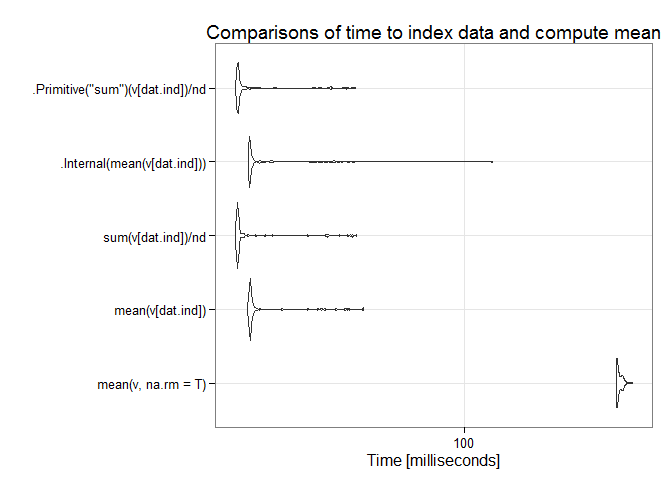
\includegraphics[width=\maxwidth]{figure/benchmarks1-1} 
\begin{kframe}\begin{alltt}
\hlkwa{if} \hlstd{(no.knit)} \hlkwd{dev.off}\hlstd{()}
\end{alltt}
\end{kframe}
\end{knitrout}

\begin{knitrout}
\definecolor{shadecolor}{rgb}{0, 0.169, 0.212}\color{fgcolor}\begin{kframe}
\begin{alltt}
\hlstd{mb2} \hlkwb{<-} \hlkwd{microbenchmark}\hlstd{(}\hlkwd{mean}\hlstd{(v[dat.ind]),} \hlkwd{sum}\hlstd{(v[dat.ind])}\hlopt{/}\hlstd{nd,} \hlkwd{mean}\hlstd{(d),} \hlkwd{sum}\hlstd{(d)}\hlopt{/}\hlstd{nd,}
    \hlkwc{times} \hlstd{=} \hlnum{1000}\hlstd{)}
\hlstd{mb2}
\end{alltt}
\begin{verbatim}
## Unit: milliseconds
##                expr       min        lq      mean    median        uq
##    mean(v[dat.ind]) 11.839516 14.043738 16.112048 14.159742 14.775524
##  sum(v[dat.ind])/nd 11.639541 12.543934 14.728460 12.647030 13.069682
##             mean(d)  2.937099  2.956692  3.059285  2.990902  3.045327
##           sum(d)/nd  1.478502  1.490320  1.566962  1.502760  1.543657
##         max neval
##  125.081989  1000
##  137.833982  1000
##    5.506281  1000
##    4.805907  1000
\end{verbatim}
\begin{alltt}
\hlkwa{if} \hlstd{(no.knit)} \hlkwd{png}\hlstd{(}\hlstr{"../plots/benchmark2.png"}\hlstd{,} \hlkwc{width} \hlstd{=} \hlnum{2000}\hlstd{,} \hlkwc{height} \hlstd{=} \hlnum{1600}\hlstd{,} \hlkwc{res} \hlstd{=} \hlnum{200}\hlstd{)}
\hlkwd{autoplot}\hlstd{(mb2)} \hlopt{+} \hlkwd{theme_bw}\hlstd{()} \hlopt{+} \hlkwd{labs}\hlstd{(}\hlkwc{title} \hlstd{=} \hlstr{"Comparisons of time to compute mean"}\hlstd{,}
    \hlkwc{y} \hlstd{=} \hlstr{"Function"}\hlstd{)}
\end{alltt}
\end{kframe}
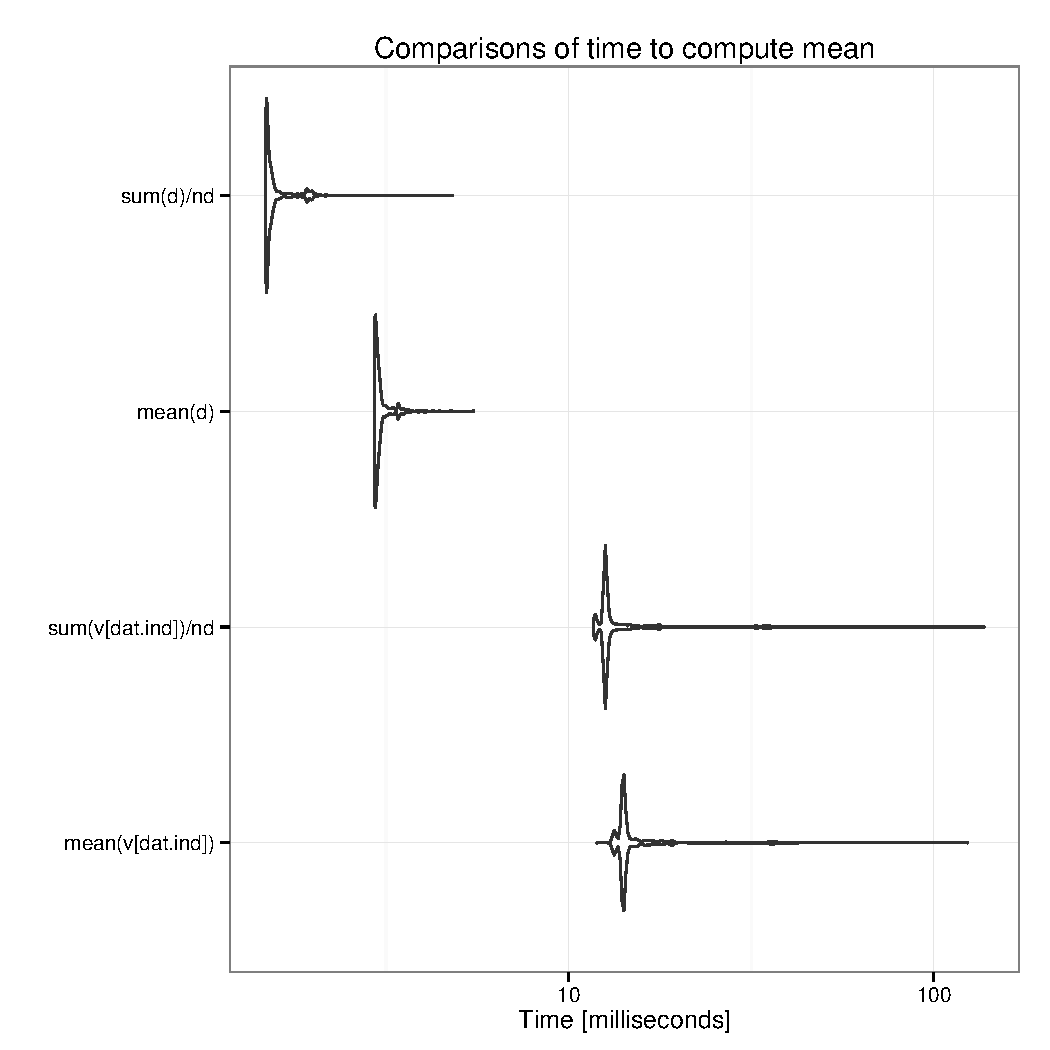
\includegraphics[width=\maxwidth]{figure/benchmarks2-1} 
\begin{kframe}\begin{alltt}
\hlkwa{if} \hlstd{(no.knit)} \hlkwd{dev.off}\hlstd{()}
\end{alltt}
\end{kframe}
\end{knitrout}

\end{document}
